% !TEX root = ../report.tex
\subsection{Brokered Authentication}

\begin{figure}[H]
\centering
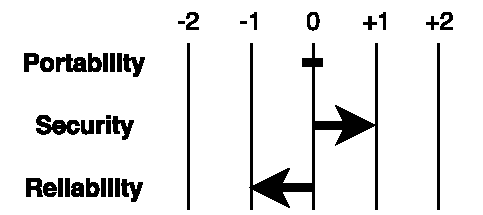
\includegraphics[scale=0.7]{6-evaluation/images/brokered_auth_frm.pdf}
\caption{Force Resolution Map for Brokered Authentication pattern.}
\label{fig:brokered-auth-frm}
\end{figure}

Reliability is ensured because if the user cannot push/pull, an error message is
prompt. In that way, the user is notified in case of a failure in his
authentication. (see definition of Reliability in the Shared Repository Pattern
evaluation).

However, there is also a drawback in the reliability because the centralized
authorization service can be a single point of failure. It may need to be online
and available, otherwise the client can't get his token. If the brokered
authentication becomes unavailable, the registry and the client can't
communicate with each other. Redundant and back-up authentication broker are the
example solutions of this problem.

Security is ensured because the registry and the client do not communicate
directly. The Bearer token is a barrier of protection between the two
components. However security tokens must be signed by the authentication broker.
If they are not, their integrity cannot be verified. This could result in
attackers trying to issue false tokens.

Portability isn't affected by the use of this pattern.

Figure \ref{fig:brokered-auth-frm} concludes the contribution of this pattern.
